\section{Multivariate analysis}

The event selection described in~\Cref{sec:event_selection} only
serves as a preselection with the intention that selected events
follow the expected topology of the signal and that basic kinematic
requirements, ensuring trigger efficiencies are in saturation, are
fulfilled.

The non-resonant and resonant production of SM Higgs boson pairs have
distinct kinematic properties that can be used to reject backgrounds
in the signal region. An example that is independent of the production
mode of SM Higgs boson pairs is the invariant mass of the \bbbar pair
and the \hadhad which can be reconstructed. A number of reconstructed
quantities can be defined that offer discrimination power to
distinguish between the various signals and backgrounds.

Multivariate methods are employed to exploit the discrimination power
of multiple reconstructed quantities and their correlations to
classify events regarding their signal- and
background-likeness. Depending on the search different methods are
used.

The search of non-resonant \HH production in the SM uses Boosted
Decision Trees and Neural Networks to distinguish between signal and
background in the \hadhad and \lephad channel, respectively. When
searching for resonant \HH production in BSM scenarios, multiple mass
hypotheses for the scalar resonance decaying into SM Higgs boson pairs
are considered. The signal event kinematics are therefore dependent on
the mass of the resonance, \mX, and as a result the classification
task continuously varies as a function of \mX. This is in contrast to
the former case where the kinematic properties of signal events are
fixed. Classification tasks that vary as a function of a parameter,
for example the resonance mass, can be performed by \emph{Parametric
  Neural Networks} (PNN), first introduced to HEP
in~\cite{Baldi:2016fzo}. PNN provide a single classifier that is able
to handle multiple classification tasks, while being able to smoothly
interpolate the parameter to values not seen during training.

The scores provided by these multivariate classification methods,
hereafter called MVA scores, are later used as a discriminant in the
maximum likelihood fit to extract the signal of interest and set upper
limits on signal strengths and cross-sections. No further selections
are applied to events entering the signal extraction procedure such
that the preselection regions are also the signal regions in the
respective channels.

In~\Cref{sec:mva_discriminating variables} the choice of
discriminating variables to classify signal and background processes
will be motivated. Afterwards, the training and optimisation of the
classifiers used to extract non-resonant signal is described
in~\Cref{sec:mva_smbdt}. Finally, \Cref{sec:mva_pnn} will explain the
interpolation properties of PNN as well as the training and
optimisation procedures used. \todo{Variable importance?}


\subsection{Cross validation method}
\label{sec:mva_crossvalidation}

Many machine learning algorithms, due to their ability to approximate
large classes of functions, are susceptible to fitting statistical
fluctuations in the data that are used to train a model. As a result,
predictions of performance characteristics of the model based on the
training data might not generalise to previously unseen data. In
extreme cases, frequently called overfitting, the performance of the
model evaluated on an independent dataset starts to degrade when
further increasing the capacity of the model~\cite{hastie09}.

When using multivariate methods in measurements or searches for new
physics, it has to be ensured that the methods are evaluated on a
dataset that was not used for training or model selection (the process
of choosing the model to fit), thus providing an estimator of the
generalised performance. In this analysis, events are categorised
according to their event number into even- and odd-numbered events,
yielding an even- and odd-fold, respectively. The training and model
selection can proceed by using one of the two folds withholding the
remaining fold for later evaluation. This procedure is applied twice
by using each fold for training once.

After model selection and training, the models are evaluated by
applying the model trained on the even-fold on odd-numbered events and
the model trained on the odd-fold on even-numbered events. This
approach, which is called two-fold \emph{cross
  validation}~\cite{hastie09,bishop06}, provides an unbiased
evaluation of the MVA scores using the entirety of the available
dataset. The same evaluation method is applied to signal region data
recorded by the ATLAS detector, which is not part of the training
procedure.

Similar to the biased predictions obtained when evaluating
multivariate methods on datasets used for training, the process of
model selection needs to be performed on a dataset that is independent
of the one used for final evaluation of the
method~\cite{cawley10}. Model selection is the process of choosing a
particular configuration of the algorithm, for example input variables
and other hyperparameters, based on a metric indicating the
performance of the model.

The model selection is performed by using five-fold cross validation
(CV), which is a generalisation of the two-fold approach described
previously to a larger number of subdivisions, separately on the even-
and the odd-numbered events. This approach effectively nests a
five-fold CV inside the a two-fold CV and is therefore called
\emph{nested cross validation}\todo{cite \cite{stone74}?}.

\Cref{fig:cross_validation} shows a schematic description of one step
of the nested cross validation approach. \todo{Continue: 5-folds
  average metric / stddev of metric}

\begin{figure}[htbp]
  \centering

  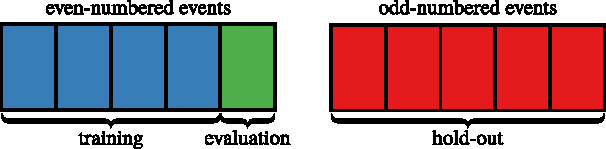
\includegraphics[scale=1]{mva/kfold}

  \caption{Five-fold cross validation approach for model selection on
    even-numbered events. The separation of events into disjoint
    subsets (folds) is indicated by rectangles. The purpose of the
    subset is denoted below. A single step out of a total of five, the
    number of possible assignments of the evaluation fold, is
    shown. The hold-out dataset is not used for model selection.}
  \label{fig:cross_validation}
\end{figure}


\subsection{Discriminating variables}
\label{sec:mva_discriminating variables}

The set of variables provided to multivariate classification methods
is crucial to its performance in distinguishing between
classes.\todo{More intro.}

The initial choice of variables for the \hadhad and \lephad channels
was based on a previous publication by the ATLAS collaboration in the
same search channel using a partial Run~2
dataset~\cite{HIGG-2016-16-witherratum}. This choice was verified for
the analysis employing the full Run~2 dataset by removing variables
not contributing to the classification performance and testing
variables that were not included in the earlier publication.










Discriminating variables were rechecked (in \hadhad) from previous
publication and found to be all significant except for MET centrality.




The discriminating variables used: \mMMC, \mBB, \mHH, \dRtautau, \dRbb.





A summary of the discriminating variables used for signal extraction
is shown in~\Cref{tab:mva_inputvars}. The same sets of variables are
used to extract the non-resonant and resonant production of \HH.

\begin{table}[htbp]
  \centering

  \missingfigure{Table of input variables}

  \caption{Discriminating variables used to extract the non-resonant
    and resonant \HH signals in the \hadhad, \lephad SLT, and \lephad
    LTT channels.}
  \label{tab:mva_inputvars}
\end{table}



\subsection{Extraction of the non-resonant signal using Boosted
  Decision Trees in the \hadhad channel}
\label{sec:mva_smbdt}

TMVA

\todo[inline]{Optimisation}

Random grid search

\todo[inline]{Performance?}





\subsection{Extraction of resonant signals with parametric neural networks}
\label{sec:mva_pnn}

Signal spectra connected to one or more physics parameters.

Input parameter: resonance mass \mX

Input parameter + input variables are inputs to the NN

Standardised by subtracting median and dividing by interquartile range.

Keras, Tensorflow, lwtnn




\todo[inline]{Optimisation}
\todo[inline]{Performance: Detuning studies}


\subsection{Others?}

\todo[inline]{Variable ranking}


%%% Local Variables:
%%% mode: latex
%%% TeX-master: "../../phd_thesis"
%%% End:
